% \begin{frame}{Objetivos de la asignatura}
%     \centering
%     \begin{tikzpicture}
%         \node at (0,3.7) {\tiny \bf {Usuario}} ;
%         \node[inner sep=0pt] (user) at (0,3) {
%             
\includegraphics[width=1.3cm]{img/user.png}
%         };

%         \node at (3,3.7) {\tiny \bf {Aplicaci\'on}} ;
%         \node[inner sep=0pt] (desktop) at (3,3) {
%             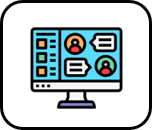
\includegraphics[width=1.3cm]{img/desktop.png}
%         };

%         \node at (6,3.7) {\tiny \bf {SGBDR}} ;
%         \node[inner sep=0pt] (dbms) at (6,3) {
%             
\includegraphics[width=1.3cm]{img/dbms.png}
%         };

%         \node at (9,3.7) {\tiny \bf {Base de datos}} ;
%         \node[inner sep=0pt] (database) at (9,3) {
%             
\includegraphics[width=1.3cm]{img/sqldb.png}
%         };

%         \draw[<->,thick] (user.east) -- (desktop.west);
%         \draw[<->,thick] (desktop.east) -- (dbms.west);
%         \draw[<->,thick] (dbms.east) -- (database.west);

%         \node<2>[circle, color=red, draw, inner xsep = 1cm] at (9,3.15) {};
%     \end{tikzpicture}

%     \vspace{20pt}
%     \begin{block}<2>{Proporcionar un conjunto de m\'etodos y herramientas para:}
%         \begin{enumerate}
%             \item Dise\~nar e implementar bases de datos correctas
%             \item Evaluar la calidad de bases de datos espec\'ificas
%         \end{enumerate}
%     \end{block}


% \end{frame}

\begin{frame}{Objetivos de la asignatura}
    \begin{block}{Bases de datos relacionales}
        \begin{itemize}
            \item<1-> Orientadas a almacenar datos estructurados (datos tabulares)
            \item<2-> Basadas en el modelo relacional (modelo matem\'atico de datos)
            \item<3-> Permiten el procesamiento transaccional de datos
            \item<4-> Base de los sistemas de informaci\'on para la generaci\'on de conocimiento
        \end{itemize}
    \end{block}

    \begin{block}<5->{Proporcionar un conjunto de m\'etodos y herramientas para:}
        \begin{itemize}
            \item<6-> Dise\~nar e implementar bases de datos correctas
            \item<7-> Evaluar la calidad de bases de datos espec\'ificas
            \item<8-> Identificar la vigencia del modelo relacional y sus limitaciones
        \end{itemize}        
    \end{block}
\end{frame}